%*****************************************************************
%   Vzorec za pisanje diplomskega dela,
%   ki vsebuje navodila za izdelavo diplomskega dela
%
%   UNIVERZA V LJUBLJANI
%   Fakulteta za računalništvo in informatiko
%
%   Pripravila: Peter.Peer@fri.uni-lj.si
%               Franc.Solina@fri.uni-lj.si
%*****************************************************************

\documentclass[12pt,a4paper,openany,twoside]{book}

%Uporabljeni paketi
\RequirePackage{pdf14}
\usepackage{cmap}
\usepackage[utf8]{inputenc}
\usepackage{type1ec}
\usepackage[T1]{fontenc}
\usepackage{graphicx,epsfig}
\usepackage[slovene]{babel}
\usepackage{cite}
\usepackage{enumitem}
\usepackage{amsmath}
%\usepackage{url}
\usepackage[pdftex,colorlinks,citecolor=black,filecolor=black,linkcolor=black,urlcolor=black]{hyperref}
\usepackage[top=2cm, bottom=3cm, inner=3cm, outer=2cm]{geometry}
\usepackage{fancyvrb}
\usepackage{incgraph}
\usepackage[a-1b]{pdfx}
%\usepackage[backend=bibtex]{biblatex}

%\addbibresource{magisterij.bib}

%Nastavitev glave in repa strani
\pagestyle{myheadings}

% stil odstavkov
\setlength{\parindent}{0cm}
\setlength{\parskip}{5mm plus2mm minus2mm}

%%%%%%%%%%%%%%%%%%%%%%%%%%%%%%%%%%%%%%%%%%%%%%%%%%%%%%%%%%%%%%%%%
%% ccBeamer 0.1, 2007-07-02                                   %%
%% Written by Sebastian Pipping <webmaster@hartwork.org>      %%
%% ---------------------------------------------------------- %%
%% Licensed under Creative Commons Attribution-ShareAlike 3.0 %%
%% http://creativecommons.org/licenses/by-sa/3.0/             %%
%%%%%%%%%%%%%%%%%%%%%%%%%%%%%%%%%%%%%%%%%%%%%%%%%%%%%%%%%%%%%%%%


%% Images
\newcommand{\CcImageBy}[1]{%
	
\includegraphics[scale=#1]{creative_commons/cc_by_30.pdf}%
}
\newcommand{\CcImageCc}[1]{%
	
\includegraphics[scale=#1]{creative_commons/cc_cc_30.pdf}%
}
\newcommand{\CcImageDevNations}[1]{%
	
\includegraphics[scale=#1]{creative_commons/cc_dev_nations_30.pdf}%
}
\newcommand{\CcImageNc}[1]{%
	
\includegraphics[scale=#1]{creative_commons/cc_nc_30.pdf}%
}
\newcommand{\CcImageNd}[1]{%
	
\includegraphics[scale=#1]{creative_commons/cc_nd_30.pdf}%
}
\newcommand{\CcImagePd}[1]{%
	
\includegraphics[scale=#1]{creative_commons/cc_pd_30.pdf}%
}
\newcommand{\CcImageSa}[1]{%
	
\includegraphics[scale=#1]{creative_commons/cc_sa_30.pdf}%
}
\newcommand{\CcImageSampling}[1]{%
	
\includegraphics[scale=#1]{creative_commons/cc_sampling_30.pdf}%
}
\newcommand{\CcImageSamplingPlus}[1]{%
	
\includegraphics[scale=#1]{creative_commons/cc_sampling_plus_30.pdf}%
}


%% Groups
\newcommand{\CcGroupBy}[1]{% zoom
	\CcImageBy{#1}%
}
\newcommand{\CcGroupByNc}[2]{% zoom, gap
	\CcImageBy{#1}\hspace*{#2}\CcImageNc{#1}%
}
\newcommand{\CcGroupByNcNd}[2]{% zoom, gap
	\CcImageBy{#1}\hspace*{#2}\CcImageNc{#1}\hspace*{#2}\CcImageNd{#1}%
}
\newcommand{\CcGroupByNcSa}[2]{% zoom, gap
	\CcImageBy{#1}\hspace*{#2}\CcImageNc{#1}\hspace*{#2}\CcImageSa{#1}%
}
\newcommand{\CcGroupByNd}[2]{% zoom, gap
	\CcImageBy{#1}\hspace*{#2}\CcImageNd{#1}%
}
\newcommand{\CcGroupBySa}[2]{% zoom, gap
	\CcImageBy{#1}\hspace*{#2}\CcImageSa{#1}%
}
\newcommand{\CcGroupDevNations}[1]{% zoom
	\CcImageDevNations{#1}%
}
\newcommand{\CcGroupNcSampling}[2]{% zoom, gap
	\CcImageNc{#1}\hspace*{#2}\CcImageSampling{#1}%
}
\newcommand{\CcGroupPd}[1]{% zoom
	\CcImagePd{#1}%
}
\newcommand{\CcGroupSampling}[1]{% zoom
	\CcImageSampling{#1}%
}
\newcommand{\CcGroupSamplingPlus}[1]{% zoom
	\CcImageSamplingPlus{#1}%
}


%********************************************
% kratice, simboli
\newcommand{\abbrlabel}[1]{\makebox[3cm][l]{\textbf{#1}\ \dotfill}}
\newenvironment{abbreviations}{\begin{list}{}{\renewcommand{\makelabel}{\abbrlabel}}}{\end{list}}
%********************************************

\begin{document}

%********************************************
% platnica
\thispagestyle{empty} 
\begin{center}
             {\large UNIVERZA V LJUBLJANI\\
                     FAKULTETA ZA RAČUNALNIŠTVO IN INFORMATIKO\\}
\vspace{3cm} {\large Iztok Jeras}\\
\vspace{2cm} {\large \textbf{Predslike 2D celičnih avtomatov}}\\
\vspace{2cm} {MAGISTRSKO DELO\\ NA UNIVERZITETNEM ŠTUDIJU}\\
\vfill       {\Large Ljubljana, 2016}
\end{center}
\newpage
\ \thispagestyle{empty}
\newpage
%********************************************

%********************************************
% stran 1 med uvodnimi listi
\thispagestyle{empty} 
\begin{center}
             {\large UNIVERZA V LJUBLJANI\\
                     FAKULTETA ZA RAČUNALNIŠTVO IN INFORMATIKO\\}
\vspace{3cm} {\large Iztok Jeras}\\
\vspace{2cm} {\large \textbf{Predslike 2D celičnih avtomatov}}\\
\vspace{2cm} {MAGISTRSKO DELO\\ NA UNIVERZITETNEM ŠTUDIJU}\\
\vspace{2cm} {\Large Mentor: prof. dr. Branko Šter}
\vfill       {\Large Ljubljana, 2016}
\end{center}
\newpage
\ \thispagestyle{empty}
\newpage
%********************************************

%********************************************
% stran 2 med uvodnimi listi
\thispagestyle{empty}

\vspace*{5cm}
{\small \noindent
To magistrsko delo je ponujeno pod licenco \textit{Creative Commons Attribution-ShareAlike 4.0 International}
\footnote{http://creativecommons.org/licenses/by-sa/4.0/} ali v slovenščini \textit{priznanje avtorstva in deljenje pod enakimi pogoji 4.0 mednarodna}
\footnote{http://www.ipi.si/sl/creative-commons-cc/o-uporabi-licence}. Po želji se lahko uporabnik poslužuje novejše različice.
To pomeni, da se tako besedilo, slike, grafi in druge sestavine dela kot tudi rezultati magistrskega dela lahko prosto distribuirajo,
reproducirajo, uporabljajo, dajejo v najem, priobčujejo javnosti in predelujejo, pod pogojem, da se jasno in vidno navede avtorja in naslov tega
dela in da se v primeru spremembe, preoblikovanja ali uporabe tega dela v svojem delu, lahko distribuira predelava le pod
licenco, ki je enaka tej.
Uporabljena je mednarodna licenca, čeprav obstaja verzija prilagojena za slovenski pravni red, to pa zato, ker slovenska verzija ni vzdrževana.
Podrobnosti licence so dostopne na spletni strani \url{http://creativecommons.org}
ali na Inštitutu za intelektualno lastnino, Streliška 1, 1000 Ljubljana.
\begin{center}

\includegraphics[width=5cm]{by-sa.png}
\end{center}
}

\vspace*{1.5cm}
{\small \noindent
Izvorna koda programske opreme, razvite za potrebe magistrskega dela, je ponujena pod licenco \textit{Unlicense} \footnote{http://unlicense.org/}.
To pomeni, da se lahko prosto uporablja, distribuira in/ali predeluje, brez kakšnih koli obveznosti.
Avtor se odpoveduje vsem pravicam in tako omogoča uporabnikom izvorne kode, da se izognejo preverjanju pravnih obveznosti.
}

\begin{center} 
\ \\ \vfill
{\em Besedilo je oblikovano z urejevalnikom besedil \LaTeX.\\
Slike in grafi so narisani s pomočjo programa za vektorske ilustracije Inkscape \footnote{https://inkscape.org}.}
\end{center}

\newpage
\ \thispagestyle{empty}
\newpage
%********************************************

% stran 3 med uvodnimi listi
\incgraph[documentpaper][width=\paperwidth,height=\paperheight]{original_izdane_teme_magistrskega_dela.jpg}
%
\includepdf{original_izdane_teme_magistrskega_dela.pdf}
%\thispagestyle{empty}
%Namesto te strani {\bf vstavite} original izdane teme magistrskega dela s podpisom mentorja in dekana ter žigom fakultete, ki ga magistrant
%dvigne v študent\-skem referatu,  preden odda izdelek v vezavo!
%\newpage

%********************************************
% stran 4 med uvodnimi listi je prazna 
\ \thispagestyle{empty}
\newpage

%********************************************
% stran 5 med uvodnimi listi

\thispagestyle{empty}

\vspace*{2cm}
\begin{center}
{\Large \textbf{IZJAVA O AVTORSTVU \\ \vspace{0.5cm} magistrskega dela}}
\end{center}
\vspace{1cm}

Spodaj podpisani \textbf{Iztok Jeras},
z vpisno številko \textbf{63030393},
sem avtor magistrskega dela z naslovom:

\vspace{1cm}
\hspace{1cm}\textbf{Predslike 2D celičnih avtomatov}
\vspace{1cm}

S svojim podpisom zagotavljam, da:
\begin{itemize}
\item sem magistrsko delo izdelal samostojno pod vodstvom mentorja \textbf{prof. dr. Branka Štera},
\item so elektronska oblika magistrskega dela, naslova (slov., angl.), povzetka (slov., angl.) ter ključne besede (slov., angl.) identični s tiskano obliko magistrskega dela
\item in soglašam z javno objavo elektronske oblike magistrskega dela v zbirki »Dela FRI«.
\end{itemize}

\vspace{3cm}
V Ljubljani, dne 30. avgust 2016 \hfill Podpis avtorja:
\newpage 

%********************************************
% stran 6 med uvodnimi listi je prazna pri dvostranskem tiskanju
\ \thispagestyle{empty}
\newpage

%********************************************
% stran 7 med uvodnimi listi

\chapter*{Zahvala}
\thispagestyle{empty}
Zahvaljujem se prof. dr. Andreju Dobnikarju za pomoč pri pisanju člankov
o algoritmih za štetje in izpis predslik pri enodimenzionalnih celičnih avtomatih.
\newpage

%********************************************
% stran 8 med uvodnimi listi je prazna pri dvostranskem tiskanju
\ \thispagestyle{empty}
\newpage

%********************************************

\renewcommand\thepage{} 
\tableofcontents 
\renewcommand\thepage{\arabic{page}}

\thispagestyle{empty}

%********************************************

\chapter*{Seznam uporabljenih kratic in simbolov}

\thispagestyle{empty}

% simboli

\begin{abbreviations}
\item[1D] enodimenzionalen
\item[2D] dvodimenzionalen
\item[3D] tridimenzionalen
\item[CA] cellular automata (celični avtomat)
\item[GoL] Conway's Game of Life (Conwayeva igra življenja)
\item[GoE] Garden of Eden (rajski vrt)
\item[trid] okolica CA, sestavljena iz treh celic na heksagonalni mreži
\item[quad] okolica CA, sestavljena iz štirih celic na kvadratni mreži

\item[\(C\)] poljubna konstanta
\item[\(S\)] nabor stanj celice
\item[\(|S|\)] število možnih stanj celice
\item[\(c\)] stanje posamezne celice (celoštevilska vrednost)
\item[\(c_{x,y}\)] vrednost celice na koordinatah \((x,y)\) znotraj 2D polja celic
\item[\(c^t\)] vrednost celice v sedanjosti
\item[\(c^{t+1}\)] vrednost celice v prihodnosti (en korak)
\item[\(N_x\)] velikost pravokotnega 2D polja celic v dimenziji X
\item[\(N_y\)] velikost pravokotnega 2D polja celic v dimenziji Y
\item[\(N\)] število celic v 2D polju
\item[\(M_x\)] velikost pravokotne 2D okolice celice v dimenziji X
\item[\(M_y\)] velikost pravokotne 2D okolice celice v dimenziji Y
\item[\(m\)] število celic v 2D okolici
\item[\(n\)] stanje okolice posamezne celice (celoštevilska vrednost)
\item[\(n_{x,y}\)] vrednost okolice celice na koordinatah \((x,y)\) znotraj 2D polja celic
\item[\(n^{t-1}\)] vrednost okolice celice v preteklosti (en korak)
\item[\(n^t\)] vrednost okolice celice v sedanjosti
\item[\(f\)] tranzicijska funkcija, ki definira časovno evolucijo avtomata
\item[\(f^{-1}\)] obratna tranzicijska funkcija
\item[\(o_x\)] prekrivanje okolic v dimenziji X
\item[\(o_y\)] prekrivanje okolic v dimenziji Y
\item[\(o_{xy}\)] prekrivanje okolic v diagonalni smeri
\end{abbreviations}

%\cleardoublepage

\clearpage{\pagestyle{empty}\cleardoublepage}

%********************************************
%zacno se glavni listi, ki so numerirani z arabskimi stevilkami

\setcounter{page}{1}
\pagenumbering{arabic}

\chapter*{Povzetek}

\addcontentsline{toc}{chapter}{Povzetek}

Medtem ko je računanje predslik 1D celičnih avtomatov dobro raziskan in
podrobno dokumentiran problem, je to področje pri 2D celičnih avtomatih manj raziskano.
Za 1D problem poznamo algoritme za štetje in izpis predslik s
procesno zahtevnostjo linearno odvisno od velikosti problema.
Možno je tudi določiti, ali je 1D celični avtomat reverzibilen in
kakšen je regularen jezik vseh stanj brez predslik.
Pri 2D problemu sicer poznamo nekaj algoritmov za iskanje predslik,
vendar so slabo teoretično raziskani.
Vemo tudi, da je problem reverzibilnosti 2D celičnih avtomatov na splošno neodločljiv.

Mreža predslik, ki sem jo razvil za potrebe analize predslik 1D celičnih avtomatov,
se je izkazala za praktično orodje pri razlagi algoritmov in pri dokazovanju njihove pravilnosti.
Tukaj opišem, kako se mrežo predslik tvori za 2D celične avtomate.
Če je bila ta mreža za 1D problem navaden graf, je za 2D problem razširjena v tretjo dimenzijo.
Predslike so namesto poti v grafu ploskve na mreži.
Robni pogoj se spremeni iz uteži za vozlišča, ki zaključujejo pot v 1D problemu,
v uteži za sklenjeno pot okoli ploskve predslike v 2D problemu.

Pri razvoju algoritma se je izkazalo, da štetja predslik 2D celičnega avtomata
ni mogoče izvesti v linearni odvisnosti od velikosti problema.
Zahtevnost podanega algoritma narašča eksponentno z velikostjo problema v eni dimenziji.
Podani algoritem se ne razlikuje dosti od obstoječih.
Celični avtomat razdeli na vrstice in išče predslike za posamezno vrstico od prve do zadnje.
Vrstične rezultate nato združi v rešitev za celoten 2D problem.
Podobno kot pri algoritmu za 1D probleme, je analiza razdeljena v dva prehoda.
V prvem prehodu po vrsticah algoritem prešteje predslike,
v drugem opcijskem prehodu pa predslike izpiše.
Drugi prehod poteka v obratni smeri kakor prvi prehod,
tudi procesiranje posamezne vrstice poteka iz drugega zornega kota.

Glavni napredek algoritma vidim v uporabi učinkovitih rešitev za 1D problem pri analizi vrstic ter
v uporabi progresivnega kodiranja vmesnih rezultatov, kar lahko zmanjša porabo pomnilnika.

\vspace{1.3cm}
\noindent
{\large \bf Ključne besede:}

\vspace{0.5cm}
\noindent
celični avtomati, predslike, predhodniki, računska zahtevnost, reverzibilnost, rajski vrt, Conwayeva igra življenja, trid, quad
\newpage

% prazna stran
\ \thispagestyle{empty}
\newpage

\chapter*{Abstract}

\addcontentsline{toc}{chapter}{Abstract}

While computing preimages of 1D cellular automata is a well researched and documented problem,
for 2D cellular automata there is less research available.
For the 1D problem we know algorithms for counting and listing preimages
where computational complexity is a linear function of the size of the problem.
It is possible to determine whether a 1D cellular automaton is reversible,
and what is the Garden of Eden sequence regular language.
For the 2D problem we know a few algorithms,
but they are poorly theoretically researched.
We also know that the reversibility problem is
in general undecidable for 2D cellular automata.

The preimage network, first developed for 1D cellular automata,
was proved to be a useful tool for explaining algorithms and for constructing proofs.
Here I explain how to construct the preimage network for 2D cellular automata.
While for the 1D problem this network is a normal graph,
for 2D it was extended into the third dimension.
Preimages are transformed from paths in the graph in 1D into surfaces on the network in 2D.
Edge conditions are transformed from weights for vertices ending a path in the 1D problem
into weights for the closed path around a preimage surface in the 2D problem.

While developing the algorithm, it proved impossible
to count preimages of 2D cellular automata
with processing requirements growing linearly with problem size.
Instead, processing requirements grow exponentially
with the size in one of the dimensions.
The described algorithm does not differ much from the existing ones.
The cellular automaton is split into rows,
the preimage list is first determined for each row from the first to the last.
The row results are then combined into the result for the whole 2D problem.
In a similar fashion to the 1D approach,
the algorithm splits into two passes.
In the first pass preimages are counted,
in the second optional pass preimages are listed.
The second pass is performed in the opposite direction,
while rows are also observed from the opposite side.

I see the main advantage of the described algorithm
in using existing solutions for row processing.
Solutions proved to be effective in solving the 1D problem.
Using progressive encoding of intermediate solutions
also enables reducing memory consumption.

\vspace{1.3cm}
\noindent
{\large \bf Key words:}

\vspace{0.5cm}
\noindent
cellular automata, preimages, predecessors, ataviser, computational complexity, reversibility, Garden of Eden, Conway's Game of Life, trid, quad
\newpage

% prazna stran
\ \thispagestyle{empty}
\newpage

%********************************************

\chapter{Uvod}

\section{Celični avtomati kot model vesolja}

Ker lahko vsak univerzalen sistem modelira vsak drug univerzalen sistem, lahko predpostavimo,
da lahko z univerzalnimi celičnimi avtomati (CA) modeliramo vesolje. Samo modeliranje vesolja
je še izven našega dosega, poizkuša pa se vsaj približati teorijo CA in teoretično fiziko.
S strani informacijske teorije in termodinamike je predvsem zanimiv model gravitacije
kakor entropijske sile (Entropic gravity \cite{Verlinde2010}), ki predpostavlja, da je
3D vesolje projekcija procesov, ki se odvijajo na 2D ploskvi. Z druge strani pa CA tudi omogočajo
opazovanje abstraktnega kopiranja informacij (replikacija) in evolucije \cite{Salzberg2004}.
Oba sta pomembna informacijska pojava v našem vesolju.

\section{Informacijska dinamika}

Informacijsko dinamiko CA se najpogosteje opisuje samo kakor reverzibilno ali ireverzibilno,
obstaja tudi nekaj člankov, ki opazujejo entropijo sistema.
Pri reverzibilnem avtomatu se vsa informacija ohranja, vsako stanje ima natanko eno prihodnost in eno preteklost.
Za reverzibilen celični avtomat lahko tudi definiramo pravilo oziroma funkcijo,
s katero preprosto procesiramo avtomat v preteklost namesto prihodnost.
Za reverzibilne CA je torej računanje predslik (preteklosti)
trivialno in ne potrebuje tukaj opisanega algoritma.
Za ireverzibilne CA tako reverzno pravilo ne obstaja.
Trenutno stanje ima lahko nobeno, eno, ali več predslik.
Za take avtomate pravimo, da s časom izgubljajo informacijo,
ker ne koremo enolično določiti preteklega stanja.

Pogosto je tudi opazovanje dinamike delcev pri GoL (Game of Life ali slovensko igra življenja) (slika \ref{gospers_glider_gun})
\footnote{Gospers glider gun. Wikipedia. Dostop Avgust 2016, na naslovu \url{https://commons.wikimedia.org/wiki/File:Gospers_glider_gun.gif}}
in elementarnem pravilu 110 (slika \ref{ca110-interaction2})
\footnote{CA 110 interaction 2. Wikipedia. Dostop Avgust 2016, na naslovu \url{https://en.wikipedia.org/wiki/File:Ca110-interaction2.png}}.
Pištole, trki delcev in podobni konstrukti obstajajo tako v GoL kakor pri elementarnem pravilu 110
in na splošno pri vsakem univerzalnem celičnem avtomatu.
Pištole (slika \ref{ca110-interaction2}) oddajajo delce, izvor in oddani delci skupaj rastejo v neskončnost.
S tem se informacija potrebna za opis sistema povečuje.
Slika \ref{ca110-interaction2} prikazuje dve različni interakciji med dvema delcema.
V levem primeru se delca srečata, si nekaj časa delita skupen prostor in nato nadaljujejta pot vsak zase.
V desnem primeru se delca srečata in po trku nastane nov delec.

\begin{figure}[htb]
\centerline{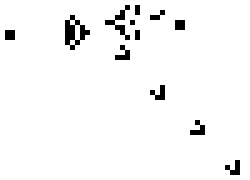
\includegraphics[width=8cm]{gospers_glider_gun}}
\caption[Gosperjeva pištola.]
{Gosperjeva pištola z nekaj izstreljenimi drsalci.}
\label{gospers_glider_gun}
\end{figure}

\begin{figure}[htb]
\centerline{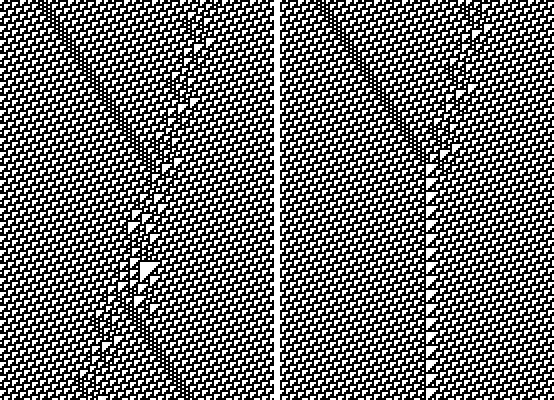
\includegraphics[width=16cm]{ca110-interaction2}}
\caption[Trk delcev v pravilu 110.]
{Trk para delcev v pravilu 110. Razlika v začetnem stanju med slikama je v razdalji (fazi) med delcema.}
\label{ca110-interaction2}
\end{figure}

Celične Avtomate sta si zamislila matematika John von Neumann in Stanislaw Ulam,
da bi lahko oblikovala teorijo univerzalnega konstruktorja
\footnote{\url{https://en.wikipedia.org/wiki/Von_Neumann_universal_constructor}},
ki je sposoben iz zapisa na traku narediti kopijo samega sebe.
Christopher Langton je vzel del univerzalnega kostruktorja in ga poenostavil v preprosto zanko
\footnote{\url{https://en.wikipedia.org/wiki/Langton\%27s_loops}},
ki kopira samo sebe na podlagi informacije zapisane v notranjosti telesa (slika \ref{langtons_loop}).

\begin{figure}[htb]
\centering
\begin{BVerbatim}
  2 2 2 2 2 2 2 2 
2 1 7 0 1 4 0 1 4 2
2 0 2 2 2 2 2 2 0 2
2 7 2         2 1 2
2 1 2         2 1 2
2 0 2         2 1 2
2 7 2         2 1 2
2 1 2 2 2 2 2 2 1 2 2 2 2 2
2 0 7 1 0 7 1 0 7 1 1 1 1 1
  2 2 2 2 2 2 2 2 2 2 2 2 2
\end{BVerbatim}
\caption[Langtonova zanka.]
{Langtonova zanka. Številke so stanja posamezne celice. Spodaj desno iz zanke raste nova zanka.}
\label{langtons_loop}
\end{figure}

Zgoraj našteti primeri nekako opisujejo informacijsko dinamiko v CA.
Ne obstaja pa še splošna teorija dinamike informacij v CA,
ki bi dinamiko opisala kvantitativno in prostorsko.
V svojem članku \cite{JerasDobnikar2007} in prispevkih na konferencah \cite{DBLP:conf/iccS/JerasD06, DBLP:conf/automata/Jeras08, Jeras2008-pyca}
sem grafično upodobil predslike trenutnega stanja za 1D problem.
Iz upodobitve (slika \ref{network_rule110_quiescent}) je videti, da se ponekod izgubi več informacije kakor drugod,
kar kaže na možnost izpeljave splošne teorije dinamike informacij.
Na žalost se ta možnost še ni udejanila. Podobno je možno grafično upodobiti predslike 2D CA,
ter iz grafov sklepati o izgubi informacije v 2D CA.

\begin{figure}[htb]
\centerline{\psfig{figure=network_rule110_quiescent,width=16cm}}
\caption[Mreža predslik 1D CA.]
{Mreža predslik 1D CA pravilo 110 za tiho ozadje s cikličnim zaporedjem 00010011011111.
Vsaka od dveh povdarjenih poti med levim in desnim predstavlja predskiko.
V enem delu sta si predliki enaki, drugod se razlikujeta.
Laično lahko sklepamo, da se tam kjer se predliki razlikujeta izgubi 1 bit informacije.}
\label{network_rule110_quiescent}
\end{figure}

\section{Problem predslik 2D CA}

Najbolje teoretično raziskan 2D CA je GoL.
Ogromno truda je bilo vloženega v raziskovanje delcev in njihove dinamike. S pomočjo
osnovnih gradnikov je mogoče skonstruirati kompleksnejše sisteme, med katerimi so
najzanimivejši Turingov stroj \cite{Rendell2001} in univerzalni konstruktor \cite{Greene2013}.

Delci so dejansko atraktorji v razvoju CA na končni periodični mreži (torus).
Pri 1D CA se algoritmi za iskanje predslik uporabljajo za določitev atraktorjevega korita \cite{Wuensche1992}.
V vsakem CA, ki ni lokalno injektiven, se pojavljajo stanja brez predslik, imenovana GoE
(\textit{Garden of Eden} ali rajski vrt) \cite{Moore1962, Myhill1963}.
Pomensko so stanja GoE nasprotje delcev, saj se nahajajo kar
najdlje od atraktorja, na robu korita. Stanja GoE tudi privlačijo raziskovalce,
čeprav v nekoliko manjši meri kakor delci.

Največ raziskav s področja predslik GoL je bilo opravljenih ravno s ciljem iskanja stanj GoE.
S stališča algoritma za štetje predslik je stanje GoE tako stanje, ki nima nobene predslike.
Algoritem za štetje predslik je možno pretvoriti v manj zahteven algoritem za preverjanje ali je dano stanje stanje GoE,
tako da se operacije nad celimi števili pretvori v logične operacije nad Boolovimi stanji.

\section{Algoritmi za iskanje predslik}

Raziskave algoritmov sem se lotil s predpostavko, da je možno opraviti štetje z zahtevnostjo,
ki je linearno odvisna od velikosti problema \( O(N) \)  (\(N\) je število opazovanih celic).
Čeprav je to možno pri 1D problemu, se izkaže, da 2D problem ni tako preprost.
Predstavljeni so primeri, iz katerih je razvidno,
da algoritem z linearno zahtevnostjo ne more pravilno opisati vseh situacij.
Zahtevnost opisanega algoritma sicer raste eksponentno z velikostjo ene
od dimenzij polja CA \( O(C^{N_x}) \), je pa možno, da obstaja algoritem z nižjo kompleksnostjo.

Pomembno vlogo pri razvoju opisanega algoritma ima mreža predslik.
To je grafična upodobitev problema, katere cilj je lažje razumevanje problema in rešitve.
Osnova za oblikovanje mreže predslik so De Bruijnovi diagrami.
Paulina Léon in Genaro Martínez \cite{PaulinaGenaro2016}
poizkušata aplicirati De Bruijnove diagrame na 2D CA.
Doslej je bilo to orodje uporabljeno le na 1D problemih.
Točneje, opazujeta dva CA: 'Game of Life' in 'Diffusion rule',
s poudarkom na opazovanju stabilnih delcev.
Sam uporabljam De Bruijnove diagrame nekoliko drugače,
in jih tudi drugače grafično upodabljam.
Posamezen De Bruijnov diagram postane mreža predslik ene celice.
Mreže posameznih celic se nato povezujejo,
tako da na koncu opisujejo celotno polje celic.

Doslej sem že razvil napredne algoritme za izračun predslik 1D CA \cite{JerasDobnikar2007}.
Skozi zgodovino so taki algoritmi napredovali, tako da je padala njihova
računska zahtevnost in opisna/implementacijska zahtevnost.
\begin{enumerate}[noitemsep,nolistsep]
 \item 'brute force' algoritmi \( O(C^N) \)
 \item improvizirani algoritmi
 \item zasnove matematičnega modela
 \item optimalni algoritmi \( O(N) \)
\end{enumerate}
Iskanje predslik 2D CA je trenutno nekje med improvizacijo in matematičnim modelom.

Opisan algoritem na koncu primerjam z ostalimi doslej znanimi algoritmi.
Čeprav s stališča procesne zahtevnosti ne prinaša želenega napredka,
pa to, da temelji na pregledni grafični upodobitvi, daje upanje,
da bodo razne optimizacije razvidne bodočim raziskovalcem.

Celični avtomat GoL je definiran z Moorovo okolico velikosti \(3 \times 3\).
Tako velika okolica ima z \(9\) celicami \(2^9=512\) možnih stanj,
zaradi česar so ilustracije mreže predslik velike in nepregledne.
Splošno je znana manjša von Neumannova okolica velikosti \(3 \times 3\) v obliki križa iz \(5\) celic.
Z \(2^5=32\) stanji bi bile ilustracije bolj pregledne, pa obstajajo tudi okolice z manj celicami.
Toffoli \cite{Toffoli2008} je leta 2008 spodbudil raziskovalce k iskanju univerzalnosti za CA
z okolicama trid (tri celice na heksagonalnem polju) in quad (štiri celice na kvadratnem polju).
Powley \cite{Powley2008} hitro dokaže obstoj univerzalnega avtomata z okolico trid,
tako da ustvari avtomat, ki lahko s pomočjo določenega začetnega stanja
simulira poljubni 1D elementarni celični avtomat, na primer pravilo 110.
Sam sem obe okolici poznal že prej. Njuna najboljša lastnost je majhen nabor stanj okolice,
\(2^4=16\) za quad in \(2^3=8\) za trid. Za primere je bil uporabljen quad,
saj so diagrami na kvadratni mreži bolj enostavni in pregledni kakor diagrami na heksagonalni mreži.

Algoritem je implementiran kot računalniški program v jeziku C \cite{Jeras2016-algirithm}.
Knjižnica GMP \footnote{The GNU Multiple Precision Arithmetic Library \url{https://gmplib.org/}}
je uporabljena za zapis celih števil, večjih od 64 bitov.
Poleg samega algoritma za štetje in izpis predslik sem pripravil tudi
orodje za simulacijo binarnega CA z okolico quad \cite{Jeras2016-quad}.
%in orodje za prikaz poljubne mreže predslik \cite{Jeras2016-network}.
Obe orodji se lahko zažene kar v internetnem brskalniku.

V slikah je uporabljena izometrična projekcija,
saj je za potrebe analize osnovnemu 2D polju dodana tretja dimenzija,
ki opisuje prostor predslik (mreža predslik).

\chapter{Definicija 2D CA}

Predstavljena definicija 2D CA je enostavna in manj formalna
v primerjavi z definicijo 1D CA v podobnih prispevkih.
Bolj formalna definicija ni potrebna, saj se opisani problemi pri 2D CA
še ne povezujejo z drugimi vejami matematike toliko kakor pri 1D CA.

Osnovni element 2D CA je celica, ki je del polja celic.
Vsaka celica ima diskretno vrednost \(c\) iz nabora stanj celice \(S\).
Stanja so običajno kar oštevilčena.

\begin{equation}
c \in S
\quad \textrm{in} \quad
S = \{ 0, 1, \ldots, {\lvert S \rvert} -1 \}
\end{equation}

Mreža polja je lahko pravokotna, šestkotna ali celo kvazikristalna. Tukaj se
bomo omejili na pravokotno mrežo. Na splošno je velikost polja lahko neskončna,
bolj običajna pa so končna polja, definirana kakor pravokotnik velikosti \(N_x \times N_y\).
Skupno število celic v končnem polju je \(N=N_x \cdot N_y\).

Prihodnje stanje neke celice \(c_{x,y}\) na s koordinatami \((x,y)\)
je odvisno od trenutnega stanja pripadajoče okolice \(n_{x,y}\) (slika \ref{neighborhood}).
Tudi pri obliki okolice se bom omejil na pravokotnik velikosti \(M_x \times M_y\).
Število celic v okolici je \(m=M_x \cdot M_y\).
Na voljo je \({\lvert S \rvert}^m\) možnih okolic.

\begin{equation}
n \in S^m
\quad \textrm{in} \quad
S^m = \{ 0, 1, \ldots, {\lvert S \rvert}^m -1 \}
\end{equation}

Prostorski odnos med okolico in celico v prihodnjem stanju avtomata, ki jo ta okolica določa,
ni podrobno definiran. Običajno se smatra, da je celica v sredini okolice, ampak za opisani algoritem to ni
nujno pomembno. Moja implementacija algoritma celice, okolice in samo polje indeksira tako,
da je začetna ali referenčna celica v spodnjem levem kotu.

\begin{figure}[htb]
\centerline{\psfig{figure=neighborhood,width=16cm}}
\caption[Velikost okolice.]{Celica \(c_{x,y}\) in pripadajoča okolica \(n_{x,y}\) z dimenzijama \(M_x=M_y=3\).}
\label{neighborhood}
\end{figure}

Preslikava sedanje okolice \(n_{x,y}^{t}\) v prihodnjo istoležno celico \(c_{x,y}^{t+1}\) je definirana
s tranzicijsko funkcijo \(f\), ki vsaki vrednosti okolice pripiše vrednost celice:

\begin{equation}
c_{x,y}^{t+1} = f(n_{x,y}^{t})
\end{equation}

Za potrebe iskanja predslik je zanimiva obratna funkcija \(f^{-1}\), ki ob
podanem stanju trenutne celice \(c_{x,y}^{t}\) vrne množico okolic,
ki se preslikajo v to vrednost:

\begin{equation}
f^{-1}(c^{t}) = \{ n^{t-1} \in S^m \ \arrowvert \ f(n^{t-1}) = c^{t} \}
\end{equation}

Dodaten pogoj za predslike polja celic je, da se morajo okolice sosednjih celic
ujemati povsod, kjer se prekrivajo.
Opazovanje prekrivanja okolic je tudi glavni element algoritmov za iskanje predslik.

Tranzicijsko funkcijo je možno definirati s pravilom.
Pravilo \(r\) je celo število v \(S\)-iškem številskem sestavu,
kjer so cifre zaporedje vrednosti celic za vsako od \(|S|^m\) možnih okolic:

\begin{equation}
r = \sum_{n=0}^{n=|S|^m-1} |S|^n \cdot f(n)
\end{equation}
\begin{equation}
r \in \{0, 1, \ldots |S|^{|S|^m}-1\}
\end{equation}

Vseh pravil je na voljo \(|S|^{|S|^m}\).
Pri 1D elementarnih CA (\(m=3\)) je vseh pravil le 256, tako da so bila že vsa opazovana in opisana.
Za 2D CA z okolico quad (\(m=4\)) je pravil 65536, kar je nekje na meji, kar lahko raziskovalci podrobno pregledajo.
Za 2D CA z Moorovo okolico (\(m=9\)) je vseh pravil dosti preveč, da bi lahko pregledali posamično.

Podana konstrukcija mreže predslik in algoritem za izračun predslik omogočata uporabo
bolj splošne definicije. Za vsako celico je lahko definiran lasten nabor predslik \( n^{t-1} \in S^m \),
ki je na splošno neodvisen od stanja celice. Ta posplošitev je uporabljena za konstrukcijo umetnih
mrež predslik, ki poudarjajo konkretne probleme, povezane s kompleksnostjo algoritma.

Za dano polje celic velikosti \(N_x \times N_y\) in z odprtimi robovi,
je možno izračunati prihodnje stanje polja velikosti \((N_x-(M_x-1)) \times (N_y-(M_y-1))\).
V primeru, da so robovi polja ciklično zaprti (polje v obliki torusa),
pa je polje prihodnjega stanja enako veliko kakor polje sedanjega.
Podobno velja za računanje predslik. Za sedanje polje velikosti \(N_x \times N_y\)
je za odprte robove velikost polja predslik enaka \((N_x+(M_x-1)) \times (N_y+(M_y-1))\).
Za ciklične robove pa sta velikosti enaki.

\chapter{Konstrukcija mreže predslik}

Mreža predslik je grafični konstrukt, ki omogoča upodobitev posameznih pojmov
iz definicije CA, kakor ločenih grafičnih elementov. Odnosi med
temi elementi definirajo pravila, na katerih se gradijo algoritmi za iskanje
predslik.

\section{De Bruijnov diagram}

Osnovni element grafične upodobitve je De Bruijnov diagram. V osnovi ta obravnava
ciklične premike končnih zaporedij simbolov ter njihovo prekrivanje. Vozlišča v
diagramu so vsa možna končna zaporedja, povezave med njimi pa definirajo, kako se
ta zaporedja prekrivajo med seboj.

Pri 1D CA se problem neposredno preslika na De Bruijnov graf. McIntosh
in njegova skupina uporabljajo za analizo De Bruijnove grafe neposredno. Sam pa sem
razvil modificiran graf, kjer so vozlišča podvojena, in gredo poti vedno od originala
proti dvojniku (slika \ref{de_bruijn_diagram}).
To omogoča veriženje grafov in razširitev osnovnega De Bruijnovega grafa.
Medtem ko osnovni De Bruijnov graf opisuje okolico ene celice, verižen graf opisuje verigo celic.

\begin{figure}[htb]
\centerline{\psfig{figure=de_bruijn_diagram,width=12cm}}
\caption[De Bruijnov graf, pravilo 110.]
{De Bruijnov graf za elementarni 1D CA, pravilo 110.
Na levi je McIntosheva upodobitev, na desni pa moja, ki omogoča veriženje.}
\label{de_bruijn_diagram}
\end{figure}

Za potrebe opisa 2D celičnih avtomatov je bila elementom
De Bruijnovega grafa dodana nova dimenzija. Povezave med vozlišči se spremenijo
v ploskve, vozlišča pa se spremenijo v robove ploskev.
Elementi celičnega avtomata, ki se preslikajo v graf, so:
\begin{itemize}[noitemsep,nolistsep]
\item nabor vseh možnih \textbf{okolic} celice postane nabor vseh \textbf{ploskev} (slika \ref{neighborhood_surfaces})
\item nabor \textbf{prekrivanj okolic v smeri 2D dimenzij} (slika \ref{overlap_dimension_quad}) postane nabor \textbf{povezav}
\item nabor \textbf{prekrivanj okolic v diagonalni smeri} (slika \ref{overlap_diagonal_quad}) postane nabor \textbf{vozlišč}
\end{itemize}

Elemente celičnega avtomata, kot so okolice in prekrivanja okolic, je potrebno indeksirati,
tako da se lahko vsakemu elementu pripiše unikatna števna vrednost.
Vsaki okolici je pripisana zaporedna vrednost, ki je konstruirana kakor \(m\)-mestno število
v \(S\)-iškem številskem sistemu (za podane primere dvojiškem):

\begin{equation}
n = \sum_{\substack{x=0 \\ y=0}}^{\substack{x=M_x-1 \\ y=M_y-1}} |S|^{M_x y + x} \cdot c_{x,y}
\end{equation}
\begin{equation}
n \in \{0, 1, \ldots, |S|^{M_x M_y}-1\}
\end{equation}

Cifre si sledijo od spodaj levo do zgoraj desno znotraj okolice
(sliki \ref{neighborhood_index_moore} in \ref{neighborhood_index_quad}).

\begin{figure}[htb]
\centerline{\psfig{figure=neighborhood_index_moore,width=12cm}}
\caption[Indeksiranje okolice \(3 \times 3\).]{Indeksiranje okolice celice z dimenzijama \(M_x=M_y=3\).}
\label{neighborhood_index_moore}
\end{figure}

\begin{figure}[htb]
\centerline{\psfig{figure=neighborhood_index_quad,width=10cm}}
\caption[Indeksiranje okolice \(2 \times 2\).]{Indeksiranje okolice celice z dimenzijama \(M_x=M_y=2\).}
\label{neighborhood_index_quad}
\end{figure}

Celice se v smeri dimenzije X prekrivajo za ploskev velikosti \((M_x-1) \times M_y\) (sliki \ref{overlap_dimension_moore} in \ref{overlap_dimension_quad}).
To ob indeksiranju da nabor:
\begin{equation}
o_{x^-} = \sum_{\substack{x=0 \\ y=0}}^{\substack{x=M_x-2 \\ y=M_y-1}} |S|^{(M_x-1) y + x} \cdot c_{x,y}
\end{equation}
\begin{equation}
o_{x^+} = \sum_{\substack{x=1 \\ y=0}}^{\substack{x=M_x-1 \\ y=M_y-1}} |S|^{(M_x-1) y + x} \cdot c_{x,y}
\end{equation}
\begin{equation}
o_x \in \{0, 1, \ldots, |S|^{(M_x-1)M_y}-1\}
\end{equation}

Celice se v smeri dimenzije Y prekrivajo za ploskev velikosti \(M_x \times (M_y-1)\) (sliki \ref{overlap_dimension_moore} in \ref{overlap_dimension_quad}).
To ob indeksiranju da nabor:
\begin{equation}
o_{y^-} = \sum_{\substack{x=0 \\ y=0}}^{\substack{x=M_x-1 \\ y=M_y-2}} |S|^{M_x y + x} \cdot c_{x,y}
\end{equation}
\begin{equation}
o_{y^+} = \sum_{\substack{x=0 \\ y=1}}^{\substack{x=M_x-1 \\ y=M_y-1}} |S|^{M_x y + x} \cdot c_{x,y}
\end{equation}
\begin{equation}
o_y \in \{0, 1, \ldots, |S|^{M_x(M_y-1)}-1\}
\end{equation}

\begin{figure}[htb]
\centerline{\psfig{figure=overlap_dimension_moore,width=8cm}}
\caption[Prekrivaje okolic \(3 \times 3\) v smeri dimenzij X in Y.]
{Prekrivanje okolic sosednjih celic v smeri dimenzij X in Y, za velikost okolice \(M_x=M_y=3\).
Okolice se prekrivajo v 6 celicah od 9.}
\label{overlap_dimension_moore}
\end{figure}

\begin{figure}[htb]
\centerline{\psfig{figure=overlap_dimension_quad,width=8cm}}
\caption[Prekrivaje okolic \(2 \times 2\) v smeri dimenzij X in Y.]
{Prekrivanje okolic sosednjih celic v smeri dimenzij X in Y, za velikost okolice \(M_x=M_y=2\).
Okolice se prekrivajo v 2 celicah od 4.}
\label{overlap_dimension_quad}
\end{figure}

Celice se v diagonalni smeri prekrivajo za ploskev velikosti \((M_x-1) \times (M_y-1)\) (sliki \ref{overlap_diagonal_moore} in \ref{overlap_diagonal_quad}).
To ob indeksiranju da nabor:
\begin{equation}
o_{{x^-}{y^-}} = \sum_{\substack{x=0 \\ y=0}}^{\substack{x=M_x-2 \\ y=M_y-2}} |S|^{(M_x-1) y + x} \cdot c_{x,y}
\end{equation}
\begin{equation}
o_{{x^+}{y^-}} = \sum_{\substack{x=1 \\ y=0}}^{\substack{x=M_x-1 \\ y=M_y-2}} |S|^{(M_x-1) y + x} \cdot c_{x,y}
\end{equation}
\begin{equation}
o_{{x^-}{y^+}} = \sum_{\substack{x=0 \\ y=1}}^{\substack{x=M_x-2 \\ y=M_y-1}} |S|^{(M_x-1) y + x} \cdot c_{x,y}
\end{equation}
\begin{equation}
o_{{x^+}{y^+}} = \sum_{\substack{x=1 \\ y=1}}^{\substack{x=M_x-1 \\ y=M_y-1}} |S|^{(M_x-1) y + x} \cdot c_{x,y}
\end{equation}
\begin{equation}
o_{xy} \in \{0, 1, \ldots, |S|^{(M_x-1)(M_y-1)}-1\}
\end{equation}

\begin{figure}[htb]
\centerline{\psfig{figure=overlap_diagonal_moore,width=10cm}}
\caption[Prekrivanje okolic \(3 \times 3\) - diagonalno.]
{Prekrivanje okolic sosednjih celic v diagonalni smeri, za velikost okolice \(M_x=M_y=3\).
Okolice se prekrivajo v 4 celicah od 9.}
\label{overlap_diagonal_moore}
\end{figure}

\begin{figure}[htb]
\centerline{\psfig{figure=overlap_diagonal_quad,width=8cm}}
\caption[Prekrivanje okolic \(2 \times 2\) - diagonalno.]
{Prekrivanje okolic sosednjih celic v diagonalni smeri, za velikost okolice \(M_x=M_y=2\).
Okolice se prekrivajo v eni celici od 4.}
\label{overlap_diagonal_quad}
\end{figure}

Graf predslik je postavljen na kvadrat, ki predstavlja okolico \(n\).
Nad vsakim vogalom je nabor vozlišč, ki predstavljajo nabor vogalnih prekrivanj
\(o_{{x^-}{y^-}}\), \(o_{{x^+}{y^-}}\), \(o_{{x^-}{y^+}}\) in \(o_{{x^+}{y^+}}\).
Vozlišči sosednjih vogalov sta povezani, če sta del iste konfiguracije celic,
ki predstavlja povezavo. Na primer, pri okolici quad povezava za prekrivanje okolic \verb|[01]|
povezuje vozlišči \verb|[0]| in \verb|[1]| (slika \ref{network_single} levo).

Nastali graf (slika \ref{network_single} desno) ima poleg vozlišč in povezav med njimi tudi ploskve.
Ploskve bi v teoriji grafov opisali kakor zanke v grafu, z dodano omejitvijo,
da mora vsako vozlišče ali povezava v zanki pripadati drugemu prekrivanju okolic.

\begin{figure}[htb]
\centerline{\psfig{figure=network_single,width=12cm}}
\caption[Mreža ene celice.]{Mreža ene celice za binarni CA z okolico quad \(M_x=M_y=2\).}
\label{network_single}
\end{figure}

\begin{figure}[htb]
\centerline{\psfig{figure=neighborhood_surfaces,width=16cm}}
\caption[Nabor ploskev.]{Nabor ploskev za vseh 16 možnih vrednosti okolic za binarni CA z okolico quad \(M_x=M_y=2\).}
\label{neighborhood_surfaces}
\end{figure}

\section{Mreža}

Diagrame, ki opisujejo preteklost posamezne celice, je možno sestaviti v mrežo,
ki opisuje polje več celic. Nabor predslik celotnega polja je ekvivalenten naboru
vseh \textit{zveznih} ploskev, ki prekrivajo celotno polje (zahteva po prekrivanju okolic)
in ki jih je možno sestaviti iz naborov ploskev diagramov posameznih celic (zahteva po ujemanju s tranzicijsko funkcijo).

Preslikava iz zvezne ploskve v mreži predslik v konfiguracijo polja celic predslike je enolična.
Najlažje je razumeti preslikavo za okolico velikosti \(3 \times 3\).
Od vsakega odseka ploskve za posamezno celico vzamemo centralno celico,
na koncu pa dodamo še za eno celico širok rob okoli celotne ploskve.

Podani primeri uporabljajo binarni CA z okolico quad.
Za ta CA je velikost diagonalnega prekrivanja okolic ena sama celica (slika \ref{overlap_diagonal_quad});
posledično ima nabor vozlišč le dve vrednosti, ki neposredno predstavljajo
vrednosti celic v predsliki (slika \ref{network_array}).
Nabor okolic/ploskev pa obsega 16 kombinacij (slika \ref{neighborhood_surfaces}).

Pravilnost razširitve diagrama ene celice v mrežo lahko dokažemo z indukcijo.
Dokazati želimo, da je neka konfiguracija celic predslika dane sedanjosti,
\textit{če in samo če} je ta ekvivalentna zvezni ploskvi v mreži predslik.

\textbf{Prvi element:}
Iz definicije velja, da je za eno samo celico v mreži nabor ploskev enak naboru vseh predslik.
\textbf{Naslednji element:}
Obstoječi mreži predslik dodamo novo celico.
Ploskev iz nabora dodane celice se zvezno veže s ploskvijo
iz obstoječega nabora zveznih ploskev,
ko se z njo ujema v robu (vozliščema in povezavi med njima).
Robovi ploskev se ujemajo natanko v primeru, ko se ujemajo prekrivanja okolic.
Temu je tako, ker so indeksi vozlišč in povezav ekvivalentni vrednosti prekrivanj okolic.

\begin{figure}[htb]
\centerline{\psfig{figure=network_array,width=14cm}}
\caption[Mreža polja celic.]{Mreža velikosti \(N_x=3\) in \(N_y=3\) za binarni CA z okolico quad.
Poudarjena je ena zvezna ploskev in njen zvezen rob. Konfiguracija pripadajoče predslike je izpisana.}
\label{network_array}
\end{figure}

\section{Robni pogoji} 

Pri 1D CA so robni pogoji definirani na dveh koncih,
ki omejujejo končno število celic na neskončni premici.
Če je 1D CA definiran kakor poltrak, je robni pogoj samo eden.
Robni pogoj definira, katere okolice (vozlišča pri mreži predslik za 1D CA)
in s kakšnimi utežmi so na voljo ob robu.
Lahko si jih predstavljamo tudi kakor vpliv neskončnega poltraka celic,
ki sega izven roba opazovane konfiguracije.

Pri 2D CA je robni pogoj definiran kakor utež sklenjene poti okoli ploskve opazovane konfiguracije celic.
V mreži predslik za 2D CA povezave med vozlišči definirajo rob ploskve (slika \ref{network_array}).
Vsaka zvezna ploskev v mreži ima zvezen rob. Robni pogoj določa, kako je ta ploskev obravnavana,
oziroma, ali je sploh obravnavana.
Ker uporabna vrednost splošnega robnega pogoja še ni znana,
in bi splošnost izrazito povečala zahtevnost algoritma za iskanje predslik,
so tukaj vsi robovi obravnavani enako, z utežjo ena. Temu bomo rekli odprti rob,
ker ta ne definira nobenih omejitev, katere zvezne ploskve v mreži predslik
so dovoljene in katere ne.

Obstaja še en enostaven robni pogoj, ki je definiran za ciklično sklenjena končna polja CA.
Ta tip robnega pogoja tukaj ne bo obravnavan, ker še dodatno poveča kompleksnost algoritmov.
Potrebno bi bilo namreč opraviti celoten postopek iskanja predslik za vsak začetni rob posebej.
Zvezna ploskev je predslika v cikličnem polju le, če se njen začetni in končni rob ujemata.
Pojma začetnega in končnega roba sta opisana v poglavju o algoritmu.

\chapter{Algoritem za štetje in izpis predslik}

Pri 1D CA ima algoritem za štetje predslik linearno \(O(N)\) procesno in pomnilniško zahtevnost.
Posplošeno to pomeni, da se vsaka celica pojavi v izračunu samo enkrat.
Dejansko ima vsak algoritem tudi logaritmično komponento,
saj število bitov, potrebnih za zapis števcev, raste logaritmično s številom celic.
Algoritem za izpis predslik ima neizogibno eksponentno kompleksnost \(O(C^N)\),
saj maksimalno in povprečno število predslik raste eksponentno
v odvisnosti od števila celic.

Za 2D CA se je izkazalo, da obstajajo problemi, ki niso rešljivi z linearno kompleksnostjo.
Prikazani algoritem ima maksimalno eksponentno kompleksnost
v odvisnosti od posamezne dimenzije \(O(S^{N_x} S^{N_y})\).
Za sedaj je še odprta možnost za obstoj algoritma s polinomsko kompleksnostjo,
ki je nekje med linearno in eksponentno.

Opisani algoritem za štetje predslik razdeli polje celic na vrstice v dimenziji X.
Delitev po stolpcih v dimenziji Y bi bila ekvivalentna, tako da je to arbitrarna odločitev.
S stališča procesne zahtevnosti je najbolje izbrati krajšo dimenzijo.
Na podlagi zunanjega robnega pogoja algoritem najprej poišče nabor predslik za prvo vrstico.
Nabor predslik izračuna kakor uteži za robove na nasprotni strani od začetne.
Seznam robov in njihove uteži uporabi kakor vhodni robni pogoji za naslednjo vrstico.
Robne uteži, izračunane za zadnjo vrstico, predstavljajo število vseh predslik.

Algoritem za izpis predslik je nadaljevaje algoritma za štetje.
Začne z znanim številom predslik, ki ga je dalo štetje, in izpisuje predslike
po vrsticah v obratni smeri, kakor je potekalo štetje (od zadnje do prve vrstice).
Pridobljen seznam predslik je sortiran. Smer sortiranja je odvisna od smeri procesiranja.
Smer procesiranja je možno po potrebi spremeniti.

\section{Procesiranje v eni dimenziji}

Procesiranje se začne z 1D nizom celic (vrstico).
Vsaki celici v nizu pripada lastna mreža predslik, eno dimenzionalnemu nizu celic
posledično pripada povezan niz mrež predslik (slika \ref{algorithm_line} mreža \textbf{1}).
Vsak segment mreže v nizu ima svoj nabor veljavnih okolic,
ki je definiran s tranzicijsko funkcijo (ali pa je posplošeno poljuben nabor).
Na začetku se ploskve okolic sosednjih celic še ne povezujejo v
zvezno ploskev čez celoten niz. Izločiti je potrebno vse ploskve okolic,
ki se ne povezujejo z okolicami svojih sosednjih celic.

Ker se vsaka vrstica povezuje s predhodno in naslednjo vrstico, je potrebno
upoštevati tudi zveznost ploskev na prehodu med vrsticami.
Ta povezava med vrsticami je prerez opazovane ploskve na meji med vrsticama.
Vsako ploskev se obravnavana posebej in prerez se izrazi kakor robni pogoj.
Začetni robni pogoj za vsako vrstico je nabor poti med vozlišči na začetku vrstice.
Vsaka pot je obravnavana posebej (slika \ref{algorithm_line}, mreža \textbf{2}, odebeljena pot).
Začetni robni pogoj je ekvivalenten nizu prekrivanja okolic \(o_{y^-}\).

Začetni robni pogoj se aplicira tako, da se izloči iz obravnave vse ploskve,
ki nimajo skupnega roba z robno potjo (slika \ref{algorithm_line},
prehod iz mreže \textbf{1} v mrežo \textbf{2}). Po tem koraku, so vse ploskve definirane
v dveh od štirih vozlišč. Do nezveznosti lahko prihaja le še na robu, nasprotnem
začetnemu robu.

Problem se reducira iz 3D mreže in procesiranja ploskev v
2D mrežo, kjer se procesirajo poti med vozlišči (slika \ref{algorithm_line},
prehod iz mreže \textbf{2} v mrežo \textbf{3}). To je problem ekvivalenten iskanju predslik
(zvenih poti v grafu) za 1D CA, za kar se uporabi algoritem, opisan v \cite{JerasDobnikar2007}.
Rezultat so poti na prerezu med ploskvami (slika \ref{algorithm_line}, mreža \textbf{4},
končni robni pogoj je odebeljen).
Končni robni pogoj je ekvivalenten nizu prekrivanja okolic \(o_{y^+}\).

\begin{figure}[htb]
\centerline{\psfig{figure=algorithm_line,width=14cm}}
\caption[Algoritem procesiranja vrstice.]{Mreža vrstice velikosti \(N_x=3\) za binarni CA z okolico quad.
Nabor okolic/ploskev za posamezno celico je arbitraren. Izbran je tako, da poudari korake algoritma.}
\label{algorithm_line}
\end{figure}

Po procesiranju nabora vseh začetnih robnih pogojev nastane nabor vseh končnih robnih pogojev.
Ta nabor se v naslednjem koraku uporabi kakor začetni robni pogoj za naslednjo vrstico.

Nabor vseh možnih poti na meji vrstice raste eksponentno z dolžino vrstice.
Število vseh poti se izračuna iz števila celic, ki se prekrivajo med okolicama dveh vrstic.
Za deljenje po vrsticah v dimenziji X je ta nabor velikosti \( |S|^{(M_y-1)(M_x-1+N_x)} \).
Posledično kompleksnost algoritma raste eksponentno z dolžino vrstice \(O(C^{N_x})\).

\section{Procesiranje v drugi dimenziji}

V drugi dimenziji se procesira zaporedje vrstic od prve do zadnje (slika \ref{algorithm_list}).
Vsaka vrstica se začne in konča z robnim pogojem.
Ti robni pogoji so prerezi ploskev v celotni mreži predslik.
Vsako vrstico je potrebno v drugi dimenziji procesirati le enkrat, kar pomeni,
da je računska zahtevnost linearno odvisna od števila vrstic \(O(N_y)\).

Vsakemu robnemu pogoju je pripisana utež. Začetni robovi za prvo vrstico imajo pripisano utež \(w=1\).
Na splošno se lahko več začetnih robov preslika v isti končni rob ene vrstice.
Utež, pripisana končnemu robu dane vrstice, je vsota uteži vseh začetnih robnih pogojev, ki se preslikajo vanj.
Utež tako predstavlja število vseh predslik za dano in prejšnje vrstice, ki se končajo z opazovanim robom.
Robovi, s katerimi se ne konča nobena od predslik, dobijo utež \(w=0\).

Za tem, ko so procesirane vse vrstice, je znan končni rob nabora vseh zveznih ploskev na celotni mreži predslik.
Vsota uteži vseh končnih robov daje število predslik celotne mreže.

Z uporabo Boolove algebre namesto operacij množenja in seštevanja
je možno poenostaviti iskanje predslik samo na njihov obstoj za opazovani robni pogoj.
Uteži postanejo binarne vrednosti \(w \in \{0, 1\}\).

\section{Izpis predslik}

Ni nujno, da se vsak vrstični začetni pogoj preslika v nabor končnih pogojev.
Možno je, da nobena pot na končnem robu ne zadošča začetnemu pogoju in mreži predslik.
Torej po prejšnjih korakih še ni točno določeno, katere ploskve se združujejo v zvezno
celoto in katere ne. Možne so ploskve, ki prekrivajo polje samo do neke vrstice in ne naprej.

Procesiranje po drugi dimenziji poteka v obratni smeri kakor pri štetj;
začne pri zadnji vrstici in konča pri prvi vrstici (slika \ref{algorithm_list}).
Z vsakim korakom se izloča še preostale slepe poti iz mreže predslik.
Za vsako vrstico je potrebno ponovno rešiti 1D problem,
le da sta začetni in končni rob zamenjana.
Začetni rob je zaporedje prekrivanja okolic \(o_{y^+}\)
in končni rob zaporedje prekrivanja okolic \(o_{y^-}\).

Hkrati je možno še izpisovati predslike. Že na začetku procesiranja v obratni smeri
je znano število vseh predslik, kar omogoča rezervacijo pomnilnika in inicializacijo seznama predslik.
Končne robne poti in njihove uteži se uporabijo za popis tekoče vrstice celic v predslikah.
Indeks robne poti (določeno zaporedje prekrivajočih okolic) da vrednost celic v vrstici predslike.
Uteži, izračunane v smeri štetja, pa dajo število predslik,
ki jih je potrebno popisati z dano vrednostjo za vrstico celic.

Z vsakim korakom v obratni smeri se popiše nova vrstica za vsako od preštetih predslik.
Ko pride algoritem spet do začetne vrstice, so vse predslike popisane.
Hkrati so iz mreže predslik izločene vse slepe poti; ostanejo le še ploskve,
ki tvorijo zvezne ploskve na celotnem polju celic.

\begin{figure}[htb]
\centerline{\psfig{figure=algorithm_list,width=8cm}}
\caption[Algoritem za izpis predslik.]{Potek smeri procesiranja pri algoritmu za štetje in izpis predslik.}
\label{algorithm_list}
\end{figure}

Algoritem tukaj ni podrobno opisan, je pa preprosta razširitev algoritma uporabljenega
za 1D CA, opisanega v \cite{JerasDobnikar2007}. Za podrobnosti je na voljo izvorna koda \cite{Jeras2016-algirithm}.

\section{Nezmožnost procesiranja z linearno zahtevnostjo}

Podan je primer, ki kaže, zakaj procesiranje z linearno zahtevnostjo ni mogoče.

Cilj raziskovalnega dela za to raziskovalno nalogo je bil poiskati
učinkovit algoritem za iskanje predslik 2D CA. Na podlagi izkušenj z 1D CA
sem optimistično pričakoval, da bo možno problem rešiti v linearnem času.

Algoritem v linearnem času bi vsako celico obravnaval le enkrat;
na splošno bi bilo število obravnav majhna konstanta (4-krat,
če se izvaja procesiranje skozi mrežo predslik v 4 smereh/prehodih).
Tak algoritem predpostavlja, da je možno celoten nabor začetnih
robnih pogojev upoštevati hkrati v enem samem prehodu.
V koraku \textbf{2} pri procesiranju vrstice (slika \ref{algorithm_line})
bi se izločilo le ploskve, ki ne ustrezajo nobenemu od začetnih robnih pogojev.
Po nekaj poizkusih sem ugotovil, da tak algoritem ne deluje pravilno.
Vsaj nekatere poti iz nabora je potrebno upoštevati ločeno.

V podanem primeru (slika \ref{algorithm_issue}) se prvi dve vrstici zaključita z
naborom dveh končnih poti \textbf{0110} in \textbf{1111}. Če bi ti dve poti
uporabili hkrati, kakor začetni robni pogoj za naslednjo vrstico, bi dobili
enak rezultat, kakor če bi bili del robnega pogoja tudi poti \textbf{0111} in \textbf{1110}.
To pa zato, ker algoritem, ki poti ne obravnava ločeno, ne more vedeti,
kje se je pot začela, da bi jo lahko tudi pravilno zaključil.
Posledično linearen algoritem lahko vzame začetek ene od poti in ga
na vozlišču, skupnem obema potema, nadaljuje po drugi poti.
Iz mreže je razvidno, da ti dve poti nista preseka neke zvezne ploskve.
Skratka, hkratno obravnavanje celotnega nabora robnih pogojev ni možno,
kar pomeni, da je število obravnav neke celice odvisno od števila poti
in posledično od eksponenta števila celic v vrstici.

Možno je, da obstajajo drugačne optimizacije algoritma, ki lahko zmanjšajo procesno kompleksnost.

\begin{figure}[htb]
\centerline{\psfig{figure=algorithm_issue,width=14cm}}
\caption[Ovira za procesiranje z linearno zahtevnostjo.]
{Ovira za procesiranje z linearno zahtevnostjo.
Veljavni robni pogoj je odebeljen, neveljavni pa črtkan.}
\label{algorithm_issue}
\end{figure}

\chapter{Primerjava z znanimi algoritmi}

Obstoječi algoritmi za predslike 2D CA se osredotočajo izključno na GoL.
Največ algoritmov je namenjenih iskanju stanj GoE, skratka, preverjajo le
obstoj predslik in jih ne štejejo ali izpisujejo. Tukaj opisani algoritem
je zamišljen bolj univerzalno za poljuben 2D CA. Vendar univerzalnost v
praksi ni ravno pomembna, saj izven raziskovalcev GoL ni dosti zanimanja
za teoretične probleme, kakor je iskanje predslik.

\section{Iskanje stanj GoE za GoL}

Conway je leta 1970 predstavil CA po imenu GoL. Že leta 1971 sta Roger Banks in Steve Ward
predstavila prvo stanje GoE velikosti \(9 \times 33\) celic.
Odkritje je bilo objavljeno v \cite{Lifeline3}. Kasneje je Don Woods
\cite{Lifeline3, Lifeline4} s pomočjo računalnika dokazal, da je stanje res GoE.

Woodsov algoritem, tako kakor moj, deluje na vrsticah.
Začne z eno vogalno celico, katere nabor predslik je kar nabor okolic,
ki se preslikajo v stanje celice. V naslednjem koraku opazuje sosednjo celico v vrstici.
Za vse kombinacije okolic dodane celice in obstoječi nabor predslik preveri,
če se ujemajo, kjer se okolice prekrivajo. Če se ujemajo, doda sestavljeno predsliko v nabor,
sicer predslika izpade iz nabora. Ko pride algoritem do konca vrstice, nadaljuje v naslednji vrstici,
le da je sedaj prekrivanje med naborom predslik in okolico dodane celice drugačno (več sosednjih celic namesto ene).
Tako algoritem nadaljuje do konca celotne konfiguracije.
Če je končni nabor predslik prazen, je opazovana konfiguracija GoE.
Nabor predslik in s tem poraba pomnilnika in procesnega časa ostajajo
relativno majhni v primerjavi z naborom vseh stanj.
Temu je tako, ker imajo v praksi tudi deli konfiguracije GoE malo predslik.
Algoritem bi bil za konfiguracije z dosti predslikami veliko bolj pomnilniško in časovno potraten.

Nicolay Beluchenko je poiskal večje število stanj GoE velikosti \(11 \times 11\).
Sicer ne poznam vseh njegovih pristopov, ampak vsaj v enem primeru je uporabljal
podoben algoritem kakor Woods. Začel je z osrednjo celico in dodajal nove celice
v spirali okoli osrednje. Za vrednost dodane celice je uporabil tisto, ki je dala manjši nabor predslik.
Algoritem zaključi, ko z novo dodano celico ni več možno tvoriti predslik.

Leta 1974 je Duparc \cite{Duparc1972, Duparc1974} razvil drugačen algoritem,
ter z njim poiskal stanja GoE velikosti \(6 \times 122\) in \(6 \times 117\).
Algoritem uporablja teorijo končnih avtomatov in regularnih jezikov, ki je v
osnovi namenjena 1D sistemom.
Duparc je celice iz vrstice 2D polja združil v simbole regularnega jezika,
zaporedje več vrstic pa predstavlja besedo.
Duparcov algoritem ne obravnava vseh stanj vrstice enakovredno,
temveč se osredotoča na vrstice, ki zmanjšujejo nabor predslik.
Obravnavanje vseh stanj vrstic bi namreč preseglo pomnilniške sposobnosti
takratne in sedanje strojne opreme že za kratke vrstice.
Dokaže le, da za vrstice dolžine 1 ne obstaja stolpec, ki bi bil stanje GoE.
Originalni članek je v francoščini, tako da lahko algoritem opišem le na podlagi tega, kako ga opisujejo drugi.

V zadnjih letih podoben algoritem uporablja Steven Eker (CSL, SRI International, California, USA).
Dokazal je, da za pravokotne konfiguracije višine 2 in 3 ne obstajajo stanja GoE.
Dokaz za konfiguracije višine 4 z danim algoritmom še vedno presega sposobnosti sodobne strojne opreme.
Število stanj avtomata, ki opisuje jezik GoE, namreč raste eksponentno z višino.
Elker je poiskal stanja GoE velikosti \(9 \times 11\), \(8 \times 12\) in \(5 \times 83\).
Na žalost raziskovalcu delodajalec prepoveduje objavo rezultatov in podrobnosti, dokler ni opravljen interni pregled.
Tako imamo za sedaj na voljo le zgoraj navedene podatke.

Drugačen algoritem uporablja Marijn Heule \cite{Hartman2013}.
S sodelavci je zapisal vsa prekrivanja za določeno stanje v obliki binarnih enačb.
Te je nato predal orodju za reševanje SAT problemov.
Če rešitev ne obstaja, pomeni, da je stanje GoE.
Uporabljena je dodatna predpostavka, da bo rešitev zrcalno simetrična v obeh dimenzijah,
kar občutno zmanjša velikost problema.
Algoritem je še dodatno optimiziran za iskanje stanj GoE in
omogoča pregled večjega števila podobnih stanj.
Ob spremembi vrednosti ene same celice omogoča uporabo delnih rezultatov prejšnjega izračuna.
SAT metode ne poznam dobro, tako da ne morem primerjati procesne zahtevnosti.

\section{Iskanje predslik GoL na splošno}

Erlan \cite{Erlan2012} je predstavil igro, pri kateri se za dano stanje
GoL išče predslike. To dejansko ni implementacija algoritma za iskanje predslik,
je pa vzpodbudil druge k iskanju takega algoritma.

Spletna stran \url{kaggle.com} je pripravila tekmovanje \cite{kaggle2013},
kjer so morali kandidati reševati problem iskanja predslik. Podali so
nabor stanj, za katere je treba poiskati predslike, in nabor učnih sekvenc.
Pričakovali so rešitev, ki temelji na strojnem učenju ali optimizaciji,
torej fokus ni bil na eksaktni rešitvi.

Pri iskanju implementacij algoritma, sem našel Atabot \cite{Borah2013},
Celični kronometer \cite{Duxbury2013} in program baziran na SAT metodi \cite{Pigorsch2015}.
Cilj teh algoritmov sicer je iskanje predslik, ampak iskanje ni sistematično
in cilj ni nabor vseh možnih predslik.
Algoritmi se tudi poslužujejo določene hevristike pri iskanju.

\section{Polni algoritmi za štetje in izpis predslik}

Opisani algoritmi za iskanje stanj GoE, na primer Woods,
sicer omogočajo iskanje vseh predslik, ampak to ni njihov glavni namen.
Optimizirani so le za stanja GoE, kjer je predslik malo tudi za samo del konfiguracije GoE.
Predvsem niso optimizirani za splošen primer, kjer je lahko predslik veliko,
posledično so potratni s porabo pomnilnika.
Morda bi bilo možno optimizirati porabo pomnilnika,
tako da bi algoritem hranil le tekoče razlike med predslikami, namesto da jih hrani v celoti.
Nekaj podobnega počne moj algoritem, ko šteje le robove, in ne hrani celotnih predslik.

Našel sem le eno aplikacijo, ki je namenjena štetju in izpisu vseh predslik.
Bickford \cite{Bickford2012} prav tako kakor ostali procesira konfiguracijo
po vrsticah, znotraj vrstice pa lahko uporablja različne algoritme (Woods, Duparc).
Bickford opiše tudi algoritem, ki namesto procesiranja po vrsticah združuje predslike
kvadratnih podsklopov konfiguracij. Na žalost poda primerjavo med različnimi algoritmi
le kakor procesni čas za posamezno implementacijo, ne pa tudi bolj splošne
ocene maksimalne in povprečne procesne/pomnilniške zahtevnosti.

Našel sem še aplikacijo, napisano v jeziku APL \cite{ionreq2013}.
Dokumentacija te aplikacije ni dovolj jasna, da bi bilo očitno, kaj točno počne.
Iz primera pa sklepam, da je sposobna poiskati vse predslike.

\chapter{Sklepne ugotovitve}

Probleme, povezane z iskanjem predslik, lahko delimo v nivoje glede na zahtevnost:
\begin{enumerate}[noitemsep,nolistsep]
\item določitev, ali obstajajo predslike za dano trenutno stanje sistema
\item štetje predslik za dano trenutno stanje sistema
\item naštevanje konfiguracij predslik
\item vprašanje reverzibilnosti sistema
\item jezik vseh stanj GoE
\end{enumerate}

V magistrskem delu opišem algoritem, ki rešuje prve tri probleme.
Preostala problema sta si sorodna.
Problem reverzibilnosti je na splošno dokazano nerešljiv \cite{Kari1989}.
Problem jezika stanj GoE je za 1D preprosto rešljiv, za 2D pa je
verjetno podobno kakor vprašanje reverzibilnosti nerešljiv.

\section{Analiza 2D CA s pomočjo končnih avtomatov}

Problem jezika stanj brez predslik bi potreboval teorijo 2D formalnega jezika, ki še ne obstaja.
Kljub temu je možno zastaviti probleme, ki se jih da preslikati v končni avtomat.
Na primer, če obravnavamo vrstice kakor simbole jezika, lahko sestavimo končni avtomat.
Simboli (stanja vrstic) definirajo prehode med stanji končnega avtomata. Stanja avtomata pa
so vsi možni nabori robov vrstice. Pomembna je le prisotnost roba, ne pa tudi utež.
Poln nabor vsebuje vse možne robove, prazen nabor pa ne vsebuje nobenega roba.
Vsako zaporedje vrstic (simbolov), ki v avtomatu pelje iz polnega v prazno stanje, je konfiguracija GoE.
Zanke v takem avtomatu pa so sorodne delcem.

Opisani pristop postane nepraktičen že za kratke vrstice.
Število vseh možnih robov raste eksponentno z dolžino vrstice \(N_x\).
To število, \(|S|^{(M_y-1)(M_x-1+N_x)}\), je enako številu vseh načinov,
na katere se lahko okolici dveh vrstic prekrivata.
Stanja avtomata pa so vsi možni nabori robov.
Nabor lahko opišemo kakor binarni niz, kjer vsak bit pomeni
prisotnost ali odsotnost enega od robov.
Vseh stanj končnega avtomata je tako \(2^{ |S|^{(M_y-1)(M_x-1+N_x)} }\).
Število stanj avtomata postane neobvladljivo že za kratke vrstice.

Najkrajša beseda GoE znotraj regularnega jezika stanj GoE je tista,
ki po najkrajši poti in brez zank pripelje iz polnega v prazen nabor.
Pri 1D CA se je izkazalo, da je dolžina najkrajše besede GoE povezana s kompleksnostjo
prostorsko-časovnih vzorcev, ki se pojavljajo pri danem pravilu.
Podobno so verjetno tudi pri 2D CA konfiguracije GoE večje pri pravilih,
ki omogočajo kompleksno dinamiko delcev. Verjetno bi bilo možno to izkoristiti
za iskanje zanimivih pravil v okolici quad.

\section{Izboljšave podanega algoritma}

Implementacijo algoritma je možno izboljšati, tako da zahtevnost
ne raste tako hitro z velikostjo problema.
Za sedaj vidim samo rešitev, ki se osredotoča na povprečno zahtevnost, namesto na maksimalno zahtevnost.
Na primer, sedaj algoritem rezervira pomnilnik za uteži vseh možnih robov,
dovolj pa bi bilo, če bi bil rezerviran pomnilnik samo za robove z utežjo večjo od nič.
Sploh pri iskanju stanj GoE je robov malo v primerjavi z vsemi možnimi.
Tak pristop bi dal dosti manjšo porabo pomnilnika
in verjetno tudi znižal čas procesiranja.

Morda bi bilo možno vnaprej določiti zgornjo mejo števila ne-ničelnih robov.
To bi omogočalo zgodnjo oceno, če je izračun za dan problem izvedljiv.
Na primer, če bi v vrstičnem procesiranju obravnavali vse začetne robove hkrati,
namesto vsakega posebej, bi dobili prevelik nabor končnih robov.
Tak nabor bi vedno vseboval vse pravilne končne robove, in še nekaj napačnih.
Ampak skupno število bi bilo lahko občutno manjše od polnega nabora.
To število bi lahko uporabili za oceno porabe pomnilnika in časa.
Na ta način bi bilo možno reševati probleme, ki so na meji tega,
kar zmore sodobna strojna oprema.

Samo implementacijo algoritma je tudi možno optimizirati.
Univerzalnost algoritma, predvsem univerzalnost velikosti okolice,
prispeva dosti režijskih stroškov. Če bi bil algoritem specializiran
samo za quad ali GoL, bi se lahko izognil precej operacijam.
Podobno velja za nabor stanj celice. Za binarne CA je možno optimizirati
operacije, ki pretvarjajo 2D nize celic v cela števila in obratno.
Binarne podatke je možno kompaktno pakirati v pomnilnik.
Mogoče je tudi uporabiti logične operacije nad celo besedo celic,
namesto procesiranja vsake celice posebej.

Procesiranje v algoritmu poteka v gnezdenih zankah in v znanem vrstnem redu.
Le manjši del dostopov do pomnilnika je naključen.
Zaporednost podatkov že sama po sebi omogoča dobro optimizacijo dostopa do predpomnilnika,
tako da na tem področju ni dosti očitnih optimizacij.

\section{Dokazovanje}

Magistrska naloga je bolj skopa z dokazi.
Za 1D CA sem uporabljal neposredno dokaze iz teorije grafov,
pri 2D CA pa mreža predslik ni običajen graf,
tako da dokazovanje s teorijo grafov ni tako preprosto.
Verjetno pa je možno pretvoriti dani graf v dualno obliko s transformacijo zvezda-trikot.
Če obstaja dualna oblika grafa, kjer ni ploskev, temveč samo vozlišča in povezave,
bi jo lahko uporabili za izpeljavo in dokazovanje dejanske računske kompleksnosti problema.

%********************************************

\appendix

\chapter{De Bruijnov diagram za GoL}

Slika \ref{network_single_moore} prikazuje del De Bruijnovega diagrama za GoL.
Graf s 16 vozlišči in 64 povezavami je očitno preveč kompleksen, da bi bil primeren za razlago algoritma.
Število vseh možnih okolic (ploskev v diagramu) pa je celo 512.

\begin{figure}[htb]
\centerline{\psfig{figure=network_single_moore,width=13cm}}
\caption[Mreža ene celice za GoL.]{Mreža ene celice za binarni CA z Moorovo okolico \(M_x=M_y=3\).}
\label{network_single_moore}
\end{figure}

\chapter{Primer delovanja algoritma za CA z okolico quad}

V naslednjem primeru je prikazano štetje in iskanje predslik
za binarni CA (celica ima lahko \(2\) stanji) z okolico velikosti \(2 \times 2\)
in pravilom številka \verb|0x725A|.

Majhna konfiguracija velikosti \(2 \times 2\) je shranjena v datoteki \verb|test_2x2.cas|.
Uporabil bi večjo konfiguracijo, a na žalost ne poznam pravila,
ki bi za večjo konfiguracijo dal majhno število predslik.

Uporabljen je program \cite{Jeras2016-algirithm} z verzijo \verb|v1|.

\begin{verbatim}
$ ./ca2d_preimages 2 2 2 0x725a 2 2 test_2x2.cas
CA parameters:
  sts  : 2
  ngb  : siz={2,2}, a=4, n=16
  ovl-y: siz={1,2}, a=2, n=4
  ovl-x: siz={2,1}, a=2, n=4
  rem-y: siz={1,2}, a=2, n=4
  rem-x: siz={2,1}, a=2, n=4
  ver  : siz={1,1}, a=1, n=2
  shf-y: siz={1,1}, a=1, n=2
  shf-x: siz={1,1}, a=1, n=2

RULE = 0x725a
  tab [0] = [[0,0],[0,0]] = 0
  tab [1] = [[1,0],[0,0]] = 1
  tab [2] = [[0,1],[0,0]] = 0
  tab [3] = [[1,1],[0,0]] = 1
  tab [4] = [[0,0],[1,0]] = 1
  tab [5] = [[1,0],[1,0]] = 0
  tab [6] = [[0,1],[1,0]] = 1
  tab [7] = [[1,1],[1,0]] = 0
  tab [8] = [[0,0],[0,1]] = 0
  tab [9] = [[1,0],[0,1]] = 1
  tab [A] = [[0,1],[0,1]] = 0
  tab [B] = [[1,1],[0,1]] = 0
  tab [C] = [[0,0],[1,1]] = 1
  tab [D] = [[1,0],[1,1]] = 1
  tab [E] = [[0,1],[1,1]] = 1
  tab [F] = [[1,1],[1,1]] = 0

CA configuration siz [y↓,x→] = [2,2]:
 1 0
 0 1

NETWORK: edge weights from forward/backward direction,
         summed preimages
net [dy=0][y=0] = [1 1 1 1 1 1 1 1 ]
net [dy=0][y=1] = [2 2 0 2 3 3 0 1 ]
net [dy=0][y=2] = [0 3 5 0 0 2 7 2 ]  cnt [0] = 19
net [dy=1][y=0] = [0 4 4 0 0 4 5 2 ]  cnt [1] = 19
net [dy=1][y=1] = [2 0 3 4 2 0 1 1 ]
net [dy=1][y=2] = [1 1 1 1 1 1 1 1 ]

preimage i=0:  CA configuration siz [y↓,x→] = [3,3]:
 1 0 0
 0 0 0
 0 1 0

preimage i=1:  CA configuration siz [y↓,x→] = [3,3]:
 1 0 0
 0 0 0
 0 1 1

preimage i=2:  CA configuration siz [y↓,x→] = [3,3]:
 1 0 0
 0 0 1
 0 1 0

preimage i=3:  CA configuration siz [y↓,x→] = [3,3]:
 1 0 0
 0 0 1
 0 1 1

preimage i=4:  CA configuration siz [y↓,x→] = [3,3]:
 0 1 0
 1 1 0
 1 0 0

preimage i=5:  CA configuration siz [y↓,x→] = [3,3]:
 0 1 0
 1 1 0
 1 0 1

preimage i=6:  CA configuration siz [y↓,x→] = [3,3]:
 0 1 0
 1 1 0
 0 1 1

preimage i=7:  CA configuration siz [y↓,x→] = [3,3]:
 0 1 0
 1 1 0
 1 1 1

preimage i=8:  CA configuration siz [y↓,x→] = [3,3]:
 1 0 1
 0 0 0
 0 1 0

preimage i=9:  CA configuration siz [y↓,x→] = [3,3]:
 1 0 1
 0 0 0
 0 1 1

preimage i=10:  CA configuration siz [y↓,x→] = [3,3]:
 1 0 1
 0 0 1
 0 1 0

preimage i=11:  CA configuration siz [y↓,x→] = [3,3]:
 1 0 1
 0 0 1
 0 1 1

preimage i=12:  CA configuration siz [y↓,x→] = [3,3]:
 0 1 1
 1 1 0
 1 0 0

preimage i=13:  CA configuration siz [y↓,x→] = [3,3]:
 0 1 1
 1 1 0
 1 0 1

preimage i=14:  CA configuration siz [y↓,x→] = [3,3]:
 0 1 1
 1 1 0
 0 1 1

preimage i=15:  CA configuration siz [y↓,x→] = [3,3]:
 0 1 1
 1 1 0
 1 1 1

preimage i=16:  CA configuration siz [y↓,x→] = [3,3]:
 0 1 1
 1 1 1
 1 0 0

preimage i=17:  CA configuration siz [y↓,x→] = [3,3]:
 1 1 1
 0 0 1
 0 1 0

preimage i=18:  CA configuration siz [y↓,x→] = [3,3]:
 1 1 1
 0 0 1
 0 1 1
\end{verbatim}

%********************************************

\chapter{Don Woods opiše svoj algoritem}

Prilagam pisno izmenjavo z avtorjem \footnote{Don Woods /url{http://www.icynic.com/~don/}} prvega algoritma za iskanje predslik GoL.

\begin{Verbatim}[fontsize=\small]

Don Woods <don@icynic.com>	Thu, Jul 28, 2016 at 11:45 PM
To: iztok.jeras@gmail.com
> Dear Mr. Woods,
>
> I am developing an algorithm for computing preimages of 2D CA. It is based
> on the latest research for computig preimages of 1D CA.
> I am using the 2x2 quad neighborhood in the examples instead of the 3x3
> neighborhood used in Life.
> https://github.com/jeras/fri-magisterij (work in progress and Slovene
> language)
> https://github.com/jeras/preimages-2D (not working yet)
>
> As part of my masters thesis I have to compare my algorithm to existing
> ones.
> You are known as the first person to prove a pattern to be a Garden of Eden
> orphan in the Game of Life.
> Could you send me some references to this proof? I was looking for an
> article to reference, but a generic description (preferably written by you)
> or source code would be as good.
>
> Regards,
> Iztok Jeras
>

Oof, it's been quite a while; let me see what I can remember.

The "proof" was programmatic, i.e. I wrote a program to compute
predecessors to a given position, and the program claimed there were no
predecessors to the particular position that someone had theorised was
a Garden of Eden.  I did not have a formal proof of correctness for the
program.  (I was a teenager when I wrote it!)  I don't think I still
have the source code anywhere, I'm afraid.  (I might have a paper
printout of it somewhere but don't have time to search right now.)

The program worked by considering each cell in turn and looking at all
possible 3x3 predecessors that would produce the given state.  It then
looked at the next cell to the right, looking for 3x3 predecessors that
were consistent with the 6 overlapping cells from the other, etc.  (In
practice, the 3x3 neighborhoods were indexed so that I could quickly
find which of the 8 possible righthand extensions worked.)  When it had
a 3x(N+2) predecessor for the top row of N, it continued at the left of
the next row, then across that row, etc.  Obviously in those later rows
there was only one new predecessor cell being introduced for each new
current cell after the leftmost, so the combinatoric explosion was not
excessive, particularly since the GoE pattern by design did not have
many potential predecessors even for subsections.  I also deliberately
oriented the target pattern with the short dimension going across, so
that I more quickly reached the point of extending the predecessor one
cell at a time in later rows.

My program normally included a 1-wide border around the area being
backtracked, to ensure there were no artifacts introduced, but for the
GoE proof I restricted it to the non-empty rectangular boundary, which
I think was 9 by 33?  Thus, as I think was mentioned at the time, what
I actually demonstrated was a stronger result: there was no predecessor
that led to a state that included the GoE as a 9x33 subsection.

I hope that helps.  Let me know if you have further questions.

        -- Don Woods

Don Woods <don@icynic.com>	Tue, Aug 16, 2016 at 6:42 PM
To: iztok.jeras@gmail.com
> I found the time to read your response just now.
>
> Your description of the algorithm confirms what I imagined based on third
> party descriptions.
> Your details regarding combinatorial explosion which affects memory
> consumption and processing time were extra helpful.
>
> May I cite this email in my master thesis, since there are no other direct
> sources I would know of?
>
> Regards,
> Iztok Jeras

Permission granted.  Good luck with your thesis!

        -- Don Woods
\end{Verbatim}

%********************************************

%\addcontentsline{toc}{chapter}{\protect Dodatki}

\newpage
\addcontentsline{toc}{chapter}{Seznam slik}
\addtocontents{toc}{\protect\vspace{-2ex}}
\listoffigures

%\newpage
%\addcontentsline{toc}{chapter}{Seznam tabel}
%\listoftables

%\listofalgorithms

%********************************************

\newpage

\bibliographystyle{slplainurl}
%\bibliographystyle{apsrevSLO}
\addcontentsline{toc}{chapter}{Literatura}
\label{stran_literatura}
\bibliography{magisterij} 

%\printbibliography

\end{document}
